\documentclass[twoside]{book}

% Packages required by doxygen
\usepackage{fixltx2e}
\usepackage{calc}
\usepackage{doxygen}
\usepackage[export]{adjustbox} % also loads graphicx
\usepackage{graphicx}
\usepackage[utf8]{inputenc}
\usepackage{makeidx}
\usepackage{multicol}
\usepackage{multirow}
\PassOptionsToPackage{warn}{textcomp}
\usepackage{textcomp}
\usepackage[nointegrals]{wasysym}
\usepackage[table]{xcolor}

% Font selection
\usepackage[T1]{fontenc}
\usepackage[scaled=.90]{helvet}
\usepackage{courier}
\usepackage{amssymb}
\usepackage{sectsty}
\renewcommand{\familydefault}{\sfdefault}
\allsectionsfont{%
  \fontseries{bc}\selectfont%
  \color{darkgray}%
}
\renewcommand{\DoxyLabelFont}{%
  \fontseries{bc}\selectfont%
  \color{darkgray}%
}
\newcommand{\+}{\discretionary{\mbox{\scriptsize$\hookleftarrow$}}{}{}}

% Page & text layout
\usepackage{geometry}
\geometry{%
  a4paper,%
  top=2.5cm,%
  bottom=2.5cm,%
  left=2.5cm,%
  right=2.5cm%
}
\tolerance=750
\hfuzz=15pt
\hbadness=750
\setlength{\emergencystretch}{15pt}
\setlength{\parindent}{0cm}
\setlength{\parskip}{3ex plus 2ex minus 2ex}
\makeatletter
\renewcommand{\paragraph}{%
  \@startsection{paragraph}{4}{0ex}{-1.0ex}{1.0ex}{%
    \normalfont\normalsize\bfseries\SS@parafont%
  }%
}
\renewcommand{\subparagraph}{%
  \@startsection{subparagraph}{5}{0ex}{-1.0ex}{1.0ex}{%
    \normalfont\normalsize\bfseries\SS@subparafont%
  }%
}
\makeatother

% Headers & footers
\usepackage{fancyhdr}
\pagestyle{fancyplain}
\fancyhead[LE]{\fancyplain{}{\bfseries\thepage}}
\fancyhead[CE]{\fancyplain{}{}}
\fancyhead[RE]{\fancyplain{}{\bfseries\leftmark}}
\fancyhead[LO]{\fancyplain{}{\bfseries\rightmark}}
\fancyhead[CO]{\fancyplain{}{}}
\fancyhead[RO]{\fancyplain{}{\bfseries\thepage}}
\fancyfoot[LE]{\fancyplain{}{}}
\fancyfoot[CE]{\fancyplain{}{}}
\fancyfoot[RE]{\fancyplain{}{\bfseries\scriptsize Generated by Doxygen }}
\fancyfoot[LO]{\fancyplain{}{\bfseries\scriptsize Generated by Doxygen }}
\fancyfoot[CO]{\fancyplain{}{}}
\fancyfoot[RO]{\fancyplain{}{}}
\renewcommand{\footrulewidth}{0.4pt}
\renewcommand{\chaptermark}[1]{%
  \markboth{#1}{}%
}
\renewcommand{\sectionmark}[1]{%
  \markright{\thesection\ #1}%
}

% Indices & bibliography
\usepackage{natbib}
\usepackage[titles]{tocloft}
\setcounter{tocdepth}{3}
\setcounter{secnumdepth}{5}
\makeindex

% Hyperlinks (required, but should be loaded last)
\usepackage{ifpdf}
\ifpdf
  \usepackage[pdftex,pagebackref=true]{hyperref}
\else
  \usepackage[ps2pdf,pagebackref=true]{hyperref}
\fi
\hypersetup{%
  colorlinks=true,%
  linkcolor=blue,%
  citecolor=blue,%
  unicode%
}

% Custom commands
\newcommand{\clearemptydoublepage}{%
  \newpage{\pagestyle{empty}\cleardoublepage}%
}

\usepackage{caption}
\captionsetup{labelsep=space,justification=centering,font={bf},singlelinecheck=off,skip=4pt,position=top}

%===== C O N T E N T S =====

\begin{document}

% Titlepage & ToC
\hypersetup{pageanchor=false,
             bookmarksnumbered=true,
             pdfencoding=unicode
            }
\pagenumbering{alph}
\begin{titlepage}
\vspace*{7cm}
\begin{center}%
{\Large «deque» }\\
\vspace*{1cm}
{\large Generated by Doxygen 1.8.12}\\
\end{center}
\end{titlepage}
\clearemptydoublepage
\pagenumbering{roman}
\tableofcontents
\clearemptydoublepage
\pagenumbering{arabic}
\hypersetup{pageanchor=true}

%--- Begin generated contents ---
\chapter{Hierarchical Index}
\section{Class Hierarchy}
This inheritance list is sorted roughly, but not completely, alphabetically\+:\begin{DoxyCompactList}
\item \contentsline{section}{Deque}{\pageref{class_deque}}{}
\item \contentsline{section}{deque\+\_\+base}{\pageref{classdeque__base}}{}
\begin{DoxyCompactList}
\item \contentsline{section}{deque$<$ val\+\_\+type $>$}{\pageref{classdeque}}{}
\end{DoxyCompactList}
\item \contentsline{section}{deque\+\_\+iterator$<$ val\+\_\+type, ref, ptr $>$}{\pageref{structdeque__iterator}}{}
\item \contentsline{section}{deque\+\_\+iterator$<$ val\+\_\+type, val\+\_\+type \&, val\+\_\+type $\ast$ $>$}{\pageref{structdeque__iterator}}{}
\item \contentsline{section}{Node}{\pageref{class_node}}{}
\item \contentsline{section}{node$<$ val\+\_\+type $>$}{\pageref{structnode}}{}
\end{DoxyCompactList}

\chapter{Class Index}
\section{Class List}
Here are the classes, structs, unions and interfaces with brief descriptions\+:\begin{DoxyCompactList}
\item\contentsline{section}{\hyperlink{classdeque}{deque$<$ val\+\_\+type $>$} }{\pageref{classdeque}}{}
\item\contentsline{section}{\hyperlink{class_deque}{Deque} \\*Class implemention of iterator of deque }{\pageref{class_deque}}{}
\item\contentsline{section}{\hyperlink{classdeque__base}{deque\+\_\+base} \\*\hyperlink{class_deque}{Deque} }{\pageref{classdeque__base}}{}
\item\contentsline{section}{\hyperlink{structdeque__iterator}{deque\+\_\+iterator$<$ val\+\_\+type, ref, ptr $>$} \\*Class implemention of iterator of deque }{\pageref{structdeque__iterator}}{}
\item\contentsline{section}{\hyperlink{class_node}{Node} \\*Class of the element of deque }{\pageref{class_node}}{}
\item\contentsline{section}{\hyperlink{structnode}{node$<$ val\+\_\+type $>$} }{\pageref{structnode}}{}
\end{DoxyCompactList}

\chapter{File Index}
\section{File List}
Here is a list of all documented files with brief descriptions\+:\begin{DoxyCompactList}
\item\contentsline{section}{\hyperlink{deque_8h}{deque.\+h} \\*Implemention of the deque, supporting iterators Created by couatl on 09.\+04.\+16 }{\pageref{deque_8h}}{}
\end{DoxyCompactList}

\chapter{Class Documentation}
\hypertarget{classdeque}{}\section{deque$<$ val\+\_\+type $>$ Class Template Reference}
\label{classdeque}\index{deque$<$ val\+\_\+type $>$@{deque$<$ val\+\_\+type $>$}}
Inheritance diagram for deque$<$ val\+\_\+type $>$\+:\begin{figure}[H]
\begin{center}
\leavevmode
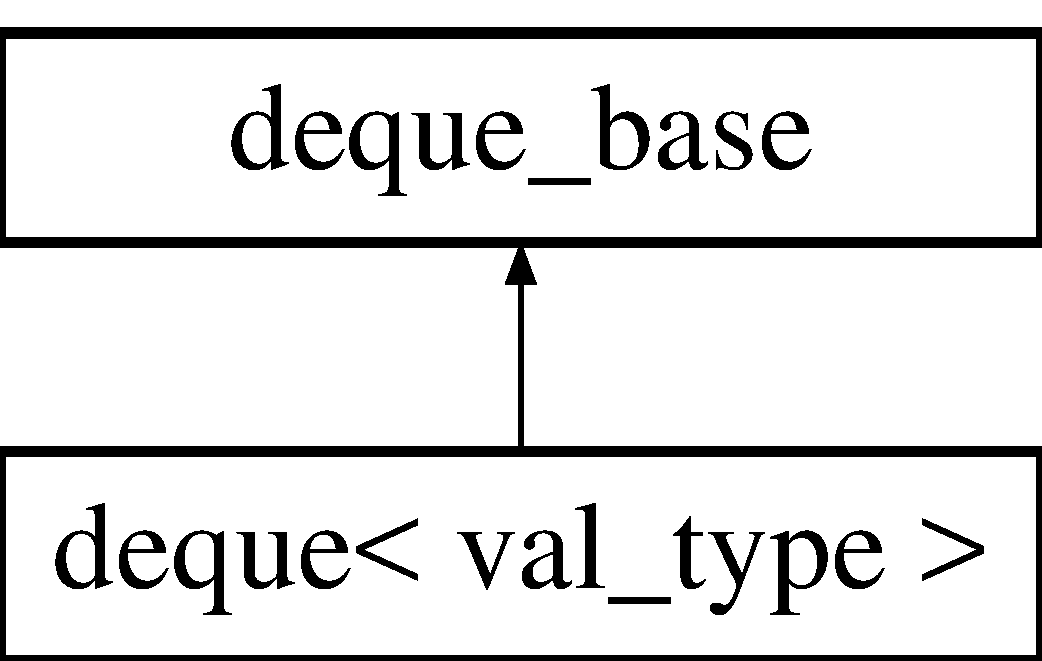
\includegraphics[height=2.000000cm]{classdeque}
\end{center}
\end{figure}
\subsection*{Public Types}
\begin{DoxyCompactItemize}
\item 
\hypertarget{classdeque_afabb1a53a41a29ed46d83221079cb5e5}{}\label{classdeque_afabb1a53a41a29ed46d83221079cb5e5} 
typedef \hyperlink{structnode}{node}$<$ val\+\_\+type $>$ {\bfseries Node}
\item 
\hypertarget{classdeque_a6af6d2c157f9cb9b85ee9a9b02ff083e}{}\label{classdeque_a6af6d2c157f9cb9b85ee9a9b02ff083e} 
typedef \hyperlink{structdeque__iterator}{deque\+\_\+iterator}$<$ val\+\_\+type, val\+\_\+type \&, val\+\_\+type $\ast$ $>$ {\bfseries iterator}
\item 
\hypertarget{classdeque_a1244237c757ffeb402c7fe2db5a70083}{}\label{classdeque_a1244237c757ffeb402c7fe2db5a70083} 
typedef \hyperlink{structdeque__iterator}{deque\+\_\+iterator}$<$ val\+\_\+type, const val\+\_\+type \&, const val\+\_\+type $\ast$ $>$ {\bfseries const\+\_\+iterator}
\end{DoxyCompactItemize}
\subsection*{Public Member Functions}
\begin{DoxyCompactItemize}
\item 
\hypertarget{classdeque_a2f2dd0e036a1daee291a01a9a03ad9d2}{}\label{classdeque_a2f2dd0e036a1daee291a01a9a03ad9d2} 
{\bfseries deque} (size\+\_\+t n)
\item 
\hypertarget{classdeque_a77986f355bfcf50434543c317b0fa370}{}\label{classdeque_a77986f355bfcf50434543c317b0fa370} 
\hyperlink{classdeque_a77986f355bfcf50434543c317b0fa370}{deque} (size\+\_\+t n, const val\+\_\+type \&var)
\begin{DoxyCompactList}\small\item\em Fill Contsructor. \end{DoxyCompactList}\item 
\hypertarget{classdeque_acb0db0be71c3bf8110742d9fae3f38e1}{}\label{classdeque_acb0db0be71c3bf8110742d9fae3f38e1} 
\hyperlink{classdeque_acb0db0be71c3bf8110742d9fae3f38e1}{deque} (\hyperlink{classdeque}{deque} \&\&move)
\begin{DoxyCompactList}\small\item\em Move Constructor. \end{DoxyCompactList}\item 
\hypertarget{classdeque_afbd8f542cd8abb0dcb03c0846e288228}{}\label{classdeque_afbd8f542cd8abb0dcb03c0846e288228} 
\hyperlink{classdeque_afbd8f542cd8abb0dcb03c0846e288228}{deque} (const \hyperlink{classdeque}{deque} \&Obj)
\begin{DoxyCompactList}\small\item\em Copy Constructor. \end{DoxyCompactList}\item 
\hypertarget{classdeque_a38f49122a62ca9156a65b201f3f02523}{}\label{classdeque_a38f49122a62ca9156a65b201f3f02523} 
\hyperlink{structdeque__iterator}{iterator} {\bfseries begin} ()
\item 
\hypertarget{classdeque_aa7e5ba5256ea1ada1420b020df653dbd}{}\label{classdeque_aa7e5ba5256ea1ada1420b020df653dbd} 
\hyperlink{structdeque__iterator}{const\+\_\+iterator} {\bfseries begin} () const
\item 
\hypertarget{classdeque_a660c98a282008bbceead5bbe77b97039}{}\label{classdeque_a660c98a282008bbceead5bbe77b97039} 
\hyperlink{structdeque__iterator}{iterator} {\bfseries end} ()
\item 
\hypertarget{classdeque_ab2b99ae02be5ad7bce0d7a5f592342be}{}\label{classdeque_ab2b99ae02be5ad7bce0d7a5f592342be} 
\hyperlink{structdeque__iterator}{const\+\_\+iterator} {\bfseries end} () const
\item 
\hypertarget{classdeque_a1791c707b5e84de39339d81c80765f58}{}\label{classdeque_a1791c707b5e84de39339d81c80765f58} 
\hyperlink{structdeque__iterator}{const\+\_\+iterator} {\bfseries cend} () const
\item 
\hypertarget{classdeque_aff9557600015f16555ae8997ca2e0ed3}{}\label{classdeque_aff9557600015f16555ae8997ca2e0ed3} 
\hyperlink{structdeque__iterator}{const\+\_\+iterator} {\bfseries cbegin} () const
\item 
\hypertarget{classdeque_ade2072ef11e762044cb3157df1932751}{}\label{classdeque_ade2072ef11e762044cb3157df1932751} 
\hyperlink{classdeque}{deque} \& {\bfseries operator=} (const \hyperlink{classdeque}{deque} \&Obj)
\item 
\hypertarget{classdeque_aa6e3f78f8aa043f605b1b723af3ff3de}{}\label{classdeque_aa6e3f78f8aa043f605b1b723af3ff3de} 
\hyperlink{classdeque}{deque} \& {\bfseries operator=} (\hyperlink{classdeque}{deque} \&\&x)
\item 
\hypertarget{classdeque_a5cedf7c96add3dbdada01afb3d1a6106}{}\label{classdeque_a5cedf7c96add3dbdada01afb3d1a6106} 
size\+\_\+t {\bfseries size} () const
\item 
\hypertarget{classdeque_aab87563431ccaaf0502d036c895294aa}{}\label{classdeque_aab87563431ccaaf0502d036c895294aa} 
void {\bfseries resize} (size\+\_\+t n)
\item 
\hypertarget{classdeque_a3c50a0c308fa95d7ebc7b6f8a7b51834}{}\label{classdeque_a3c50a0c308fa95d7ebc7b6f8a7b51834} 
bool {\bfseries empty} ()
\item 
\hypertarget{classdeque_a1e8f01b43e7d197742a1afbd758ef90d}{}\label{classdeque_a1e8f01b43e7d197742a1afbd758ef90d} 
val\+\_\+type \& {\bfseries at} (size\+\_\+t n)
\item 
\hypertarget{classdeque_ad802f6c828533e0c37dbda15d55d2c64}{}\label{classdeque_ad802f6c828533e0c37dbda15d55d2c64} 
const val\+\_\+type \& {\bfseries at} (size\+\_\+t n) const
\item 
\hypertarget{classdeque_aedc550f2b294e23a54ca35362c336c67}{}\label{classdeque_aedc550f2b294e23a54ca35362c336c67} 
val\+\_\+type \& {\bfseries front} ()
\item 
\hypertarget{classdeque_af23d9179c1f8d868de051b594d15eeca}{}\label{classdeque_af23d9179c1f8d868de051b594d15eeca} 
const val\+\_\+type \& {\bfseries front} () const
\item 
\hypertarget{classdeque_a54b65ee808502e4b1097fdb679da245c}{}\label{classdeque_a54b65ee808502e4b1097fdb679da245c} 
val\+\_\+type \& {\bfseries back} ()
\item 
\hypertarget{classdeque_aa87b733006573d31548ee2b00c4c6146}{}\label{classdeque_aa87b733006573d31548ee2b00c4c6146} 
const val\+\_\+type \& {\bfseries back} () const
\item 
\hypertarget{classdeque_aeb97a0199f6d97b25c67cdf255706f93}{}\label{classdeque_aeb97a0199f6d97b25c67cdf255706f93} 
void {\bfseries push\+\_\+front} (const val\+\_\+type \&val)
\item 
\hypertarget{classdeque_a30d370edcc61df0873dea70da51b0f21}{}\label{classdeque_a30d370edcc61df0873dea70da51b0f21} 
void {\bfseries push\+\_\+back} (const val\+\_\+type \&val)
\item 
\hypertarget{classdeque_a058b86dd11d14e61a833f745ba3b69cf}{}\label{classdeque_a058b86dd11d14e61a833f745ba3b69cf} 
void {\bfseries pop\+\_\+back} ()
\item 
\hypertarget{classdeque_ab4ddac9adc62291162d2f8ad724b2166}{}\label{classdeque_ab4ddac9adc62291162d2f8ad724b2166} 
void {\bfseries pop\+\_\+front} ()
\item 
\hypertarget{classdeque_a572cafe1303f6eadd1dbe6fc92c08a23}{}\label{classdeque_a572cafe1303f6eadd1dbe6fc92c08a23} 
void {\bfseries clear} ()
\item 
\hypertarget{classdeque_ad2e31d9c1feb97d21ad782f1c5b198ff}{}\label{classdeque_ad2e31d9c1feb97d21ad782f1c5b198ff} 
void {\bfseries assign} (size\+\_\+t n, const val\+\_\+type \&val)
\item 
\hypertarget{classdeque_a188c35dd65f58513b29f5c10eb49bd11}{}\label{classdeque_a188c35dd65f58513b29f5c10eb49bd11} 
\hyperlink{structdeque__iterator}{iterator} {\bfseries insert} (\hyperlink{structdeque__iterator}{const\+\_\+iterator} position, const val\+\_\+type \&val)
\item 
\hypertarget{classdeque_ab7f1ec9c96276c7e5b98b96d117b293b}{}\label{classdeque_ab7f1ec9c96276c7e5b98b96d117b293b} 
{\footnotesize template$<$class Input\+Iterator $>$ }\\\hyperlink{structdeque__iterator}{iterator} {\bfseries insert} (\hyperlink{structdeque__iterator}{const\+\_\+iterator} position, Input\+Iterator first, Input\+Iterator last)
\item 
\hypertarget{classdeque_a203a46e73cb25b06fd0afa309b2c0c20}{}\label{classdeque_a203a46e73cb25b06fd0afa309b2c0c20} 
val\+\_\+type \& {\bfseries operator\mbox{[}$\,$\mbox{]}} (size\+\_\+t n)
\item 
\hypertarget{classdeque_a3158df56ba89eb4ad9745cb69adf1806}{}\label{classdeque_a3158df56ba89eb4ad9745cb69adf1806} 
const val\+\_\+type \& {\bfseries operator\mbox{[}$\,$\mbox{]}} (size\+\_\+t n) const
\item 
\hypertarget{classdeque_a58cf745ac219782f3454dbaf82169b62}{}\label{classdeque_a58cf745ac219782f3454dbaf82169b62} 
void {\bfseries swap} (\hyperlink{classdeque}{deque} \&b)
\item 
\hypertarget{classdeque_ad8c083d221d558daeef4e34f5fc7d742}{}\label{classdeque_ad8c083d221d558daeef4e34f5fc7d742} 
\hyperlink{structdeque__iterator}{iterator} {\bfseries erase} (\hyperlink{structdeque__iterator}{const\+\_\+iterator} position)
\item 
\hypertarget{classdeque_a9f2317bf487ca9ab7ab011bc9d99e214}{}\label{classdeque_a9f2317bf487ca9ab7ab011bc9d99e214} 
\hyperlink{structdeque__iterator}{iterator} {\bfseries erase} (\hyperlink{structdeque__iterator}{const\+\_\+iterator} first, \hyperlink{structdeque__iterator}{const\+\_\+iterator} last)
\end{DoxyCompactItemize}
\subsection*{Static Public Member Functions}
\begin{DoxyCompactItemize}
\item 
\hypertarget{classdeque_a91b6e22358519a9e5f73d1eac2da9947}{}\label{classdeque_a91b6e22358519a9e5f73d1eac2da9947} 
static size\+\_\+t {\bfseries max\+\_\+size} ()
\end{DoxyCompactItemize}
\subsection*{Static Public Attributes}
\begin{DoxyCompactItemize}
\item 
\hypertarget{classdeque_a280e7b5814351f71d303a6b590e40b49}{}\label{classdeque_a280e7b5814351f71d303a6b590e40b49} 
static size\+\_\+t {\bfseries \+\_\+maxsize} = 100
\end{DoxyCompactItemize}
\subsection*{Additional Inherited Members}


The documentation for this class was generated from the following file\+:\begin{DoxyCompactItemize}
\item 
\hyperlink{deque_8h}{deque.\+h}\end{DoxyCompactItemize}

\hypertarget{class_deque}{}\section{Deque Class Reference}
\label{class_deque}\index{Deque@{Deque}}


Class implemention of iterator of deque.  




{\ttfamily \#include $<$deque.\+h$>$}



\subsection{Detailed Description}
Class implemention of iterator of deque. 

\begin{DoxyAuthor}{Author}
couatl 
\end{DoxyAuthor}
\begin{DoxyVersion}{Version}
1.\+0 
\end{DoxyVersion}
\begin{DoxyDate}{Date}
25/11/2016
\end{DoxyDate}
Big Boss of this project 

The documentation for this class was generated from the following file\+:\begin{DoxyCompactItemize}
\item 
\hyperlink{deque_8h}{deque.\+h}\end{DoxyCompactItemize}

\hypertarget{classdeque__base}{}\section{deque\+\_\+base Class Reference}
\label{classdeque__base}\index{deque\+\_\+base@{deque\+\_\+base}}


\hyperlink{class_deque}{Deque}.  




{\ttfamily \#include $<$deque.\+h$>$}

Inheritance diagram for deque\+\_\+base\+:\begin{figure}[H]
\begin{center}
\leavevmode
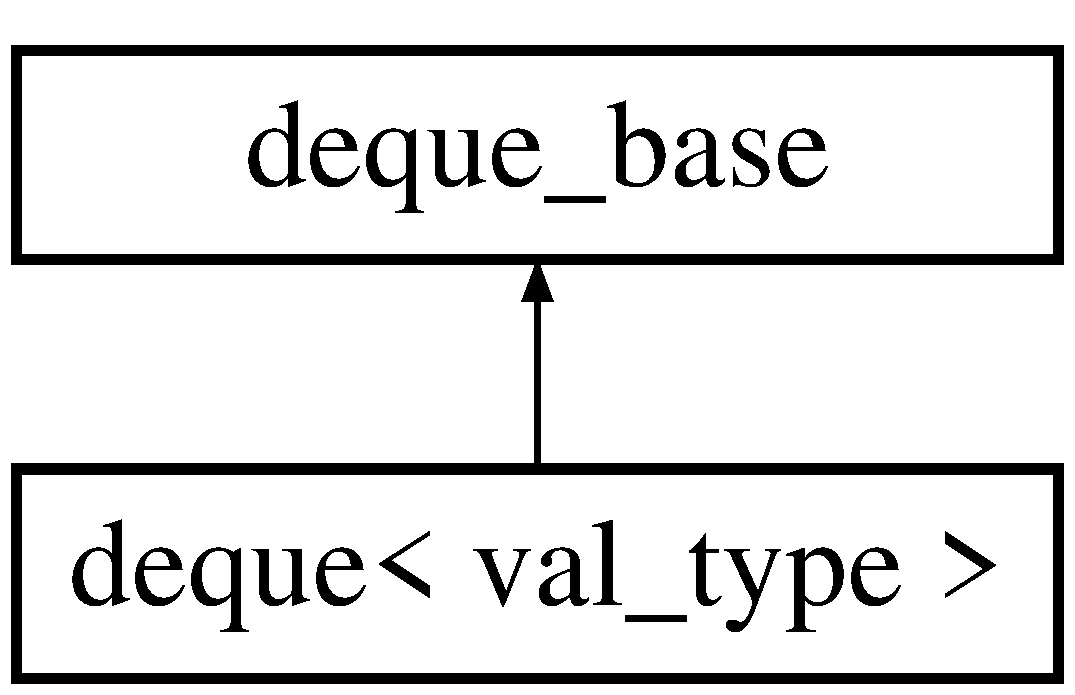
\includegraphics[height=2.000000cm]{classdeque__base}
\end{center}
\end{figure}
\subsection*{Public Attributes}
\begin{DoxyCompactItemize}
\item 
\hypertarget{classdeque__base_ad4e51927d21a0b41a078f8dd92f54895}{}\label{classdeque__base_ad4e51927d21a0b41a078f8dd92f54895} 
size\+\_\+t {\bfseries \+\_\+buff\+\_\+size}
\end{DoxyCompactItemize}


\subsection{Detailed Description}
\hyperlink{class_deque}{Deque}. 

\begin{DoxyAuthor}{Author}
couatl 
\end{DoxyAuthor}
\begin{DoxyVersion}{Version}
1.\+0.\+1 
\end{DoxyVersion}
\begin{DoxyDate}{Date}
25/11/2016 
\end{DoxyDate}


The documentation for this class was generated from the following file\+:\begin{DoxyCompactItemize}
\item 
\hyperlink{deque_8h}{deque.\+h}\end{DoxyCompactItemize}

\hypertarget{structdeque__iterator}{}\section{deque\+\_\+iterator$<$ val\+\_\+type, ref, ptr $>$ Class Template Reference}
\label{structdeque__iterator}\index{deque\+\_\+iterator$<$ val\+\_\+type, ref, ptr $>$@{deque\+\_\+iterator$<$ val\+\_\+type, ref, ptr $>$}}


Class implemention of iterator of deque.  




{\ttfamily \#include $<$deque.\+h$>$}

\subsection*{Public Types}
\begin{DoxyCompactItemize}
\item 
\hypertarget{structdeque__iterator_a9c79caebc3c261e2bb96cff829a7f715}{}\label{structdeque__iterator_a9c79caebc3c261e2bb96cff829a7f715} 
typedef \hyperlink{structnode}{node}$<$ val\+\_\+type $>$ {\bfseries Node}
\item 
\hypertarget{structdeque__iterator_ad9cb8dfbd5ae3f72ffb26133e0b80fd5}{}\label{structdeque__iterator_ad9cb8dfbd5ae3f72ffb26133e0b80fd5} 
typedef \hyperlink{structdeque__iterator}{deque\+\_\+iterator}$<$ val\+\_\+type, val\+\_\+type \&, val\+\_\+type $\ast$ $>$ {\bfseries iterator}
\item 
\hypertarget{structdeque__iterator_a6a0273686d63d0086a4cd853de840652}{}\label{structdeque__iterator_a6a0273686d63d0086a4cd853de840652} 
typedef \hyperlink{structdeque__iterator}{deque\+\_\+iterator}$<$ val\+\_\+type, const val\+\_\+type \&, const val\+\_\+type $\ast$ $>$ {\bfseries const\+\_\+iterator}
\item 
\hypertarget{structdeque__iterator_a76ad6c943c498996efacfb39d455b2ee}{}\label{structdeque__iterator_a76ad6c943c498996efacfb39d455b2ee} 
typedef \hyperlink{classdeque__base}{deque\+\_\+base} {\bfseries \+\_\+deque}
\end{DoxyCompactItemize}
\subsection*{Public Member Functions}
\begin{DoxyCompactItemize}
\item 
\hypertarget{structdeque__iterator_aa5f3b1440b64538a1979b1c266b4a1ff}{}\label{structdeque__iterator_aa5f3b1440b64538a1979b1c266b4a1ff} 
\hyperlink{structdeque__iterator_aa5f3b1440b64538a1979b1c266b4a1ff}{deque\+\_\+iterator} (\hyperlink{structnode}{Node} $\ast$base)
\begin{DoxyCompactList}\small\item\em Constructs a deque from one base node. \end{DoxyCompactList}\item 
\hypertarget{structdeque__iterator_a457004a94b85b521634813bb75a3dd1d}{}\label{structdeque__iterator_a457004a94b85b521634813bb75a3dd1d} 
\hyperlink{structdeque__iterator_a457004a94b85b521634813bb75a3dd1d}{deque\+\_\+iterator} (\hyperlink{structnode}{Node} $\ast$cur, \hyperlink{structnode}{Node} $\ast$first, \hyperlink{classdeque__base}{\+\_\+deque} $\ast$base)
\begin{DoxyCompactList}\small\item\em Constructor for initialazing a deque with begin but not with an end. \end{DoxyCompactList}\item 
\hypertarget{structdeque__iterator_ab48955425cddfe781c32b0c44e0f7121}{}\label{structdeque__iterator_ab48955425cddfe781c32b0c44e0f7121} 
\hyperlink{structdeque__iterator_ab48955425cddfe781c32b0c44e0f7121}{deque\+\_\+iterator} (\hyperlink{structnode}{Node} $\ast$cur=nullptr, \hyperlink{structnode}{Node} $\ast$first=nullptr, \hyperlink{structnode}{Node} $\ast$last=nullptr, \hyperlink{classdeque__base}{\+\_\+deque} $\ast$base=nullptr)
\begin{DoxyCompactList}\small\item\em Default constructor. \end{DoxyCompactList}\item 
\hyperlink{structdeque__iterator_acaad7042cd8df81283bd4834ba07ad30}{deque\+\_\+iterator} (const \hyperlink{structdeque__iterator}{iterator} \&T)
\begin{DoxyCompactList}\small\item\em Copy constructor. \end{DoxyCompactList}\item 
val\+\_\+type \& \hyperlink{structdeque__iterator_aa5b4c3e1340a732ea04721f69170572d}{operator$\ast$} () const
\begin{DoxyCompactList}\small\item\em Dereference operator. \end{DoxyCompactList}\item 
\hyperlink{structdeque__iterator}{deque\+\_\+iterator} \& \hyperlink{structdeque__iterator_ae15f463b8188f48d74a679935cd968ba}{operator++} ()
\begin{DoxyCompactList}\small\item\em Operator ++. \end{DoxyCompactList}\item 
\hyperlink{structdeque__iterator}{deque\+\_\+iterator} \hyperlink{structdeque__iterator_afe780014ad74f573b3eb154e91d0f66c}{operator+} (ptrdiff\+\_\+t n) const
\begin{DoxyCompactList}\small\item\em Operator +. \end{DoxyCompactList}\item 
\hyperlink{structdeque__iterator}{deque\+\_\+iterator} \hyperlink{structdeque__iterator_ab00c940267f110d87de358ba0383a9dc}{operator++} (int)
\begin{DoxyCompactList}\small\item\em Reverse operator +. \end{DoxyCompactList}\item 
\hyperlink{structdeque__iterator}{deque\+\_\+iterator} \& \hyperlink{structdeque__iterator_af9e3da57b8d1952b0ec5af9c706fefcb}{operator+=} (ptrdiff\+\_\+t n)
\begin{DoxyCompactList}\small\item\em Operator +=. \end{DoxyCompactList}\item 
\hyperlink{structdeque__iterator}{deque\+\_\+iterator} \& \hyperlink{structdeque__iterator_a9f8508814096bc20b9f00c90335f8235}{operator-\/-\/} ()
\begin{DoxyCompactList}\small\item\em Prefixed operator --. \end{DoxyCompactList}\item 
\hyperlink{structdeque__iterator}{deque\+\_\+iterator} \& \hyperlink{structdeque__iterator_ae9ba6713301a848f537cf476ecb2aacc}{operator-\/-\/} (int)
\begin{DoxyCompactList}\small\item\em Postfixed operator --. \end{DoxyCompactList}\item 
\hyperlink{structdeque__iterator}{deque\+\_\+iterator} \& \hyperlink{structdeque__iterator_ac935040db37548e0e0abefd88033dd5c}{operator-\/} (ptrdiff\+\_\+t n) const
\begin{DoxyCompactList}\small\item\em Operator -\/. \end{DoxyCompactList}\item 
\hyperlink{structdeque__iterator}{deque\+\_\+iterator} \& \hyperlink{structdeque__iterator_a1f10cb3090b780023a1454594cae75ca}{operator-\/=} (ptrdiff\+\_\+t n)
\begin{DoxyCompactList}\small\item\em Operator -\/=. \end{DoxyCompactList}\item 
val\+\_\+type $\ast$ \hyperlink{structdeque__iterator_a454c668b6534c8139be843165a5d1c9e}{operator-\/$>$} () const
\begin{DoxyCompactList}\small\item\em Operator access. \end{DoxyCompactList}\item 
\hypertarget{structdeque__iterator_aca87f964d489d8242040cd1c226f82e6}{}\label{structdeque__iterator_aca87f964d489d8242040cd1c226f82e6} 
val\+\_\+type \& {\bfseries operator\mbox{[}$\,$\mbox{]}} (ptrdiff\+\_\+t n) const
\item 
\hypertarget{structdeque__iterator_ac8c185706f46d4149e45649f85b9a4e4}{}\label{structdeque__iterator_ac8c185706f46d4149e45649f85b9a4e4} 
\hyperlink{structdeque__iterator}{deque\+\_\+iterator} \& {\bfseries operator=} (const \hyperlink{structdeque__iterator}{iterator} \&copy)
\end{DoxyCompactItemize}
\subsection*{Public Attributes}
\begin{DoxyCompactItemize}
\item 
\hypertarget{structdeque__iterator_a3ad8d3bfae3fd55a466a90e29f34e8f0}{}\label{structdeque__iterator_a3ad8d3bfae3fd55a466a90e29f34e8f0} 
\hyperlink{structnode}{Node} $\ast$ {\bfseries \+\_\+cur}
\item 
\hypertarget{structdeque__iterator_a1af9831fe2a0209c7ef3bffceb619e64}{}\label{structdeque__iterator_a1af9831fe2a0209c7ef3bffceb619e64} 
\hyperlink{structnode}{Node} $\ast$ {\bfseries \+\_\+first}
\item 
\hypertarget{structdeque__iterator_a9328ab34e070900f07e7393296d3a974}{}\label{structdeque__iterator_a9328ab34e070900f07e7393296d3a974} 
\hyperlink{structnode}{Node} $\ast$ {\bfseries \+\_\+last}
\item 
\hypertarget{structdeque__iterator_aff3cc2ab4b8c4e0ce18beb55c5176f44}{}\label{structdeque__iterator_aff3cc2ab4b8c4e0ce18beb55c5176f44} 
\hyperlink{classdeque__base}{\+\_\+deque} $\ast$ {\bfseries \+\_\+base}
\end{DoxyCompactItemize}


\subsection{Detailed Description}
\subsubsection*{template$<$class val\+\_\+type, class ref, class ptr$>$\newline
class deque\+\_\+iterator$<$ val\+\_\+type, ref, ptr $>$}

Class implemention of iterator of deque. 

\begin{DoxyAuthor}{Author}
couatl 
\end{DoxyAuthor}
\begin{DoxyVersion}{Version}
1.\+0 
\end{DoxyVersion}
\begin{DoxyDate}{Date}
25/11/2016
\end{DoxyDate}
Implemented as Random Access Iterator 

\subsection{Constructor \& Destructor Documentation}
\hypertarget{structdeque__iterator_acaad7042cd8df81283bd4834ba07ad30}{}\label{structdeque__iterator_acaad7042cd8df81283bd4834ba07ad30} 
\index{deque\+\_\+iterator@{deque\+\_\+iterator}!deque\+\_\+iterator@{deque\+\_\+iterator}}
\index{deque\+\_\+iterator@{deque\+\_\+iterator}!deque\+\_\+iterator@{deque\+\_\+iterator}}
\subsubsection{\texorpdfstring{deque\+\_\+iterator()}{deque\_iterator()}}
{\footnotesize\ttfamily template$<$class val\+\_\+type, class ref, class ptr$>$ \\
\hyperlink{structdeque__iterator}{deque\+\_\+iterator}$<$ val\+\_\+type, ref, ptr $>$\+::\hyperlink{structdeque__iterator}{deque\+\_\+iterator} (\begin{DoxyParamCaption}\item[{const \hyperlink{structdeque__iterator}{iterator} \&}]{T }\end{DoxyParamCaption})\hspace{0.3cm}{\ttfamily [inline]}}



Copy constructor. 

So basic copy constructor 
\begin{DoxyParams}[1]{Parameters}
\mbox{\tt in}  & {\em T} & Object to copy \\
\hline
\end{DoxyParams}


\subsection{Member Function Documentation}
\hypertarget{structdeque__iterator_aa5b4c3e1340a732ea04721f69170572d}{}\label{structdeque__iterator_aa5b4c3e1340a732ea04721f69170572d} 
\index{deque\+\_\+iterator@{deque\+\_\+iterator}!operator$\ast$@{operator$\ast$}}
\index{operator$\ast$@{operator$\ast$}!deque\+\_\+iterator@{deque\+\_\+iterator}}
\subsubsection{\texorpdfstring{operator$\ast$()}{operator*()}}
{\footnotesize\ttfamily template$<$class val\+\_\+type, class ref, class ptr$>$ \\
val\+\_\+type\& \hyperlink{structdeque__iterator}{deque\+\_\+iterator}$<$ val\+\_\+type, ref, ptr $>$\+::operator$\ast$ (\begin{DoxyParamCaption}{ }\end{DoxyParamCaption}) const\hspace{0.3cm}{\ttfamily [inline]}}



Dereference operator. 

\begin{DoxyReturn}{Returns}
Value of current node Dereferencing of \+\_\+cur element of this class 
\end{DoxyReturn}
\hypertarget{structdeque__iterator_afe780014ad74f573b3eb154e91d0f66c}{}\label{structdeque__iterator_afe780014ad74f573b3eb154e91d0f66c} 
\index{deque\+\_\+iterator@{deque\+\_\+iterator}!operator+@{operator+}}
\index{operator+@{operator+}!deque\+\_\+iterator@{deque\+\_\+iterator}}
\subsubsection{\texorpdfstring{operator+()}{operator+()}}
{\footnotesize\ttfamily template$<$class val\+\_\+type, class ref, class ptr$>$ \\
\hyperlink{structdeque__iterator}{deque\+\_\+iterator} \hyperlink{structdeque__iterator}{deque\+\_\+iterator}$<$ val\+\_\+type, ref, ptr $>$\+::operator+ (\begin{DoxyParamCaption}\item[{ptrdiff\+\_\+t}]{n }\end{DoxyParamCaption}) const\hspace{0.3cm}{\ttfamily [inline]}}



Operator +. 

\begin{DoxyReturn}{Returns}
Copy of the next iterator 
\end{DoxyReturn}

\begin{DoxyParams}[1]{Parameters}
\mbox{\tt in}  & {\em n} & Number to offset your current iterator Implemented based on prefixed ++. Need to Random Access Iterator \\
\hline
\end{DoxyParams}
\hypertarget{structdeque__iterator_ae15f463b8188f48d74a679935cd968ba}{}\label{structdeque__iterator_ae15f463b8188f48d74a679935cd968ba} 
\index{deque\+\_\+iterator@{deque\+\_\+iterator}!operator++@{operator++}}
\index{operator++@{operator++}!deque\+\_\+iterator@{deque\+\_\+iterator}}
\subsubsection{\texorpdfstring{operator++()}{operator++()}\hspace{0.1cm}{\footnotesize\ttfamily [1/2]}}
{\footnotesize\ttfamily template$<$class val\+\_\+type, class ref, class ptr$>$ \\
\hyperlink{structdeque__iterator}{deque\+\_\+iterator}\& \hyperlink{structdeque__iterator}{deque\+\_\+iterator}$<$ val\+\_\+type, ref, ptr $>$\+::operator++ (\begin{DoxyParamCaption}{ }\end{DoxyParamCaption})\hspace{0.3cm}{\ttfamily [inline]}}



Operator ++. 

\begin{DoxyReturn}{Returns}
Object of the next iterator Creates an element if it doesn\textquotesingle{}t exist for now 
\end{DoxyReturn}
\hypertarget{structdeque__iterator_ab00c940267f110d87de358ba0383a9dc}{}\label{structdeque__iterator_ab00c940267f110d87de358ba0383a9dc} 
\index{deque\+\_\+iterator@{deque\+\_\+iterator}!operator++@{operator++}}
\index{operator++@{operator++}!deque\+\_\+iterator@{deque\+\_\+iterator}}
\subsubsection{\texorpdfstring{operator++()}{operator++()}\hspace{0.1cm}{\footnotesize\ttfamily [2/2]}}
{\footnotesize\ttfamily template$<$class val\+\_\+type, class ref, class ptr$>$ \\
\hyperlink{structdeque__iterator}{deque\+\_\+iterator} \hyperlink{structdeque__iterator}{deque\+\_\+iterator}$<$ val\+\_\+type, ref, ptr $>$\+::operator++ (\begin{DoxyParamCaption}\item[{int}]{ }\end{DoxyParamCaption})\hspace{0.3cm}{\ttfamily [inline]}}



Reverse operator +. 

\begin{DoxyReturn}{Returns}
Copy of the offset iterator 
\end{DoxyReturn}

\begin{DoxyParams}[1]{Parameters}
\mbox{\tt in}  & {\em n} & Number to offset your current iterator Implemented based on prefixed ++. Need to Random Access Iterator \\
\hline
\end{DoxyParams}
\hypertarget{structdeque__iterator_af9e3da57b8d1952b0ec5af9c706fefcb}{}\label{structdeque__iterator_af9e3da57b8d1952b0ec5af9c706fefcb} 
\index{deque\+\_\+iterator@{deque\+\_\+iterator}!operator+=@{operator+=}}
\index{operator+=@{operator+=}!deque\+\_\+iterator@{deque\+\_\+iterator}}
\subsubsection{\texorpdfstring{operator+=()}{operator+=()}}
{\footnotesize\ttfamily template$<$class val\+\_\+type, class ref, class ptr$>$ \\
\hyperlink{structdeque__iterator}{deque\+\_\+iterator}\& \hyperlink{structdeque__iterator}{deque\+\_\+iterator}$<$ val\+\_\+type, ref, ptr $>$\+::operator+= (\begin{DoxyParamCaption}\item[{ptrdiff\+\_\+t}]{n }\end{DoxyParamCaption})\hspace{0.3cm}{\ttfamily [inline]}}



Operator +=. 

\begin{DoxyReturn}{Returns}
Offset iterator 
\end{DoxyReturn}

\begin{DoxyParams}[1]{Parameters}
\mbox{\tt in}  & {\em n} & Number to offset your current iterator Implemented based on operator + \\
\hline
\end{DoxyParams}
\hypertarget{structdeque__iterator_ac935040db37548e0e0abefd88033dd5c}{}\label{structdeque__iterator_ac935040db37548e0e0abefd88033dd5c} 
\index{deque\+\_\+iterator@{deque\+\_\+iterator}!operator-\/@{operator-\/}}
\index{operator-\/@{operator-\/}!deque\+\_\+iterator@{deque\+\_\+iterator}}
\subsubsection{\texorpdfstring{operator-\/()}{operator-()}}
{\footnotesize\ttfamily template$<$class val\+\_\+type, class ref, class ptr$>$ \\
\hyperlink{structdeque__iterator}{deque\+\_\+iterator}\& \hyperlink{structdeque__iterator}{deque\+\_\+iterator}$<$ val\+\_\+type, ref, ptr $>$\+::operator-\/ (\begin{DoxyParamCaption}\item[{ptrdiff\+\_\+t}]{n }\end{DoxyParamCaption}) const\hspace{0.3cm}{\ttfamily [inline]}}



Operator -\/. 

\begin{DoxyReturn}{Returns}
Object of the offset iterator Based on prefixed operator -- 
\end{DoxyReturn}
\hypertarget{structdeque__iterator_a9f8508814096bc20b9f00c90335f8235}{}\label{structdeque__iterator_a9f8508814096bc20b9f00c90335f8235} 
\index{deque\+\_\+iterator@{deque\+\_\+iterator}!operator-\/-\/@{operator-\/-\/}}
\index{operator-\/-\/@{operator-\/-\/}!deque\+\_\+iterator@{deque\+\_\+iterator}}
\subsubsection{\texorpdfstring{operator-\/-\/()}{operator--()}\hspace{0.1cm}{\footnotesize\ttfamily [1/2]}}
{\footnotesize\ttfamily template$<$class val\+\_\+type, class ref, class ptr$>$ \\
\hyperlink{structdeque__iterator}{deque\+\_\+iterator}\& \hyperlink{structdeque__iterator}{deque\+\_\+iterator}$<$ val\+\_\+type, ref, ptr $>$\+::operator-\/-\/ (\begin{DoxyParamCaption}{ }\end{DoxyParamCaption})\hspace{0.3cm}{\ttfamily [inline]}}



Prefixed operator --. 

\begin{DoxyReturn}{Returns}
Object of the previous iterator Creates an element if it doesn\textquotesingle{}t exist for now, even if you\textquotesingle{}re outrange (so-\/so) 
\end{DoxyReturn}
\hypertarget{structdeque__iterator_ae9ba6713301a848f537cf476ecb2aacc}{}\label{structdeque__iterator_ae9ba6713301a848f537cf476ecb2aacc} 
\index{deque\+\_\+iterator@{deque\+\_\+iterator}!operator-\/-\/@{operator-\/-\/}}
\index{operator-\/-\/@{operator-\/-\/}!deque\+\_\+iterator@{deque\+\_\+iterator}}
\subsubsection{\texorpdfstring{operator-\/-\/()}{operator--()}\hspace{0.1cm}{\footnotesize\ttfamily [2/2]}}
{\footnotesize\ttfamily template$<$class val\+\_\+type, class ref, class ptr$>$ \\
\hyperlink{structdeque__iterator}{deque\+\_\+iterator}\& \hyperlink{structdeque__iterator}{deque\+\_\+iterator}$<$ val\+\_\+type, ref, ptr $>$\+::operator-\/-\/ (\begin{DoxyParamCaption}\item[{int}]{ }\end{DoxyParamCaption})\hspace{0.3cm}{\ttfamily [inline]}}



Postfixed operator --. 

\begin{DoxyReturn}{Returns}
Object of the previous iterator Based on prefixed operator -- 
\end{DoxyReturn}
\hypertarget{structdeque__iterator_a1f10cb3090b780023a1454594cae75ca}{}\label{structdeque__iterator_a1f10cb3090b780023a1454594cae75ca} 
\index{deque\+\_\+iterator@{deque\+\_\+iterator}!operator-\/=@{operator-\/=}}
\index{operator-\/=@{operator-\/=}!deque\+\_\+iterator@{deque\+\_\+iterator}}
\subsubsection{\texorpdfstring{operator-\/=()}{operator-=()}}
{\footnotesize\ttfamily template$<$class val\+\_\+type, class ref, class ptr$>$ \\
\hyperlink{structdeque__iterator}{deque\+\_\+iterator}\& \hyperlink{structdeque__iterator}{deque\+\_\+iterator}$<$ val\+\_\+type, ref, ptr $>$\+::operator-\/= (\begin{DoxyParamCaption}\item[{ptrdiff\+\_\+t}]{n }\end{DoxyParamCaption})\hspace{0.3cm}{\ttfamily [inline]}}



Operator -\/=. 

\begin{DoxyReturn}{Returns}
Offset iterator 
\end{DoxyReturn}

\begin{DoxyParams}[1]{Parameters}
\mbox{\tt in}  & {\em n} & Number to offset your current iterator Implemented based on operator -\/ \\
\hline
\end{DoxyParams}
\hypertarget{structdeque__iterator_a454c668b6534c8139be843165a5d1c9e}{}\label{structdeque__iterator_a454c668b6534c8139be843165a5d1c9e} 
\index{deque\+\_\+iterator@{deque\+\_\+iterator}!operator-\/$>$@{operator-\/$>$}}
\index{operator-\/$>$@{operator-\/$>$}!deque\+\_\+iterator@{deque\+\_\+iterator}}
\subsubsection{\texorpdfstring{operator-\/$>$()}{operator->()}}
{\footnotesize\ttfamily template$<$class val\+\_\+type, class ref, class ptr$>$ \\
val\+\_\+type$\ast$ \hyperlink{structdeque__iterator}{deque\+\_\+iterator}$<$ val\+\_\+type, ref, ptr $>$\+::operator-\/$>$ (\begin{DoxyParamCaption}{ }\end{DoxyParamCaption}) const\hspace{0.3cm}{\ttfamily [inline]}}



Operator access. 

\begin{DoxyReturn}{Returns}
Pointer to value in the current iterator Returning pointer to the value storing in the current iterator 
\end{DoxyReturn}


The documentation for this class was generated from the following file\+:\begin{DoxyCompactItemize}
\item 
\hyperlink{deque_8h}{deque.\+h}\end{DoxyCompactItemize}

\hypertarget{class_node}{}\section{Node Class Reference}
\label{class_node}\index{Node@{Node}}


Class of the element of deque.  




{\ttfamily \#include $<$deque.\+h$>$}



\subsection{Detailed Description}
Class of the element of deque. 

\begin{DoxyAuthor}{Author}
couatl 
\end{DoxyAuthor}
\begin{DoxyVersion}{Version}
1.\+0 
\end{DoxyVersion}
\begin{DoxyDate}{Date}
25/11/2016
\end{DoxyDate}
So ordinar node of ordinar deque 

The documentation for this class was generated from the following file\+:\begin{DoxyCompactItemize}
\item 
\hyperlink{deque_8h}{deque.\+h}\end{DoxyCompactItemize}

\hypertarget{structnode}{}\section{node$<$ val\+\_\+type $>$ Struct Template Reference}
\label{structnode}\index{node$<$ val\+\_\+type $>$@{node$<$ val\+\_\+type $>$}}
\subsection*{Public Types}
\begin{DoxyCompactItemize}
\item 
\hypertarget{structnode_a51da4ba33d3e519ebf65b942dd0571c3}{}\label{structnode_a51da4ba33d3e519ebf65b942dd0571c3} 
typedef \hyperlink{classdeque__base}{deque\+\_\+base} {\bfseries \+\_\+deque}
\end{DoxyCompactItemize}
\subsection*{Public Member Functions}
\begin{DoxyCompactItemize}
\item 
\hypertarget{structnode_a019a436409b135cb62d446af7807a8fe}{}\label{structnode_a019a436409b135cb62d446af7807a8fe} 
\hyperlink{structnode_a019a436409b135cb62d446af7807a8fe}{node} (val\+\_\+type value=0, \hyperlink{structnode}{node} $\ast$next=nullptr, \hyperlink{structnode}{node} $\ast$prev=nullptr, \hyperlink{classdeque__base}{\+\_\+deque} $\ast$base=nullptr)
\begin{DoxyCompactList}\small\item\em Default constructor. \end{DoxyCompactList}\item 
\hypertarget{structnode_a92b38b0d6822f08a10912e6b5b98ae9f}{}\label{structnode_a92b38b0d6822f08a10912e6b5b98ae9f} 
\hyperlink{structnode_a92b38b0d6822f08a10912e6b5b98ae9f}{$\sim$node} ()
\begin{DoxyCompactList}\small\item\em Destructor. \end{DoxyCompactList}\end{DoxyCompactItemize}
\subsection*{Public Attributes}
\begin{DoxyCompactItemize}
\item 
\hypertarget{structnode_a10faac7d7a8c74b14071308f7f39247f}{}\label{structnode_a10faac7d7a8c74b14071308f7f39247f} 
val\+\_\+type {\bfseries \+\_\+value}
\item 
\hypertarget{structnode_a21b1a1c25784f032c41ca82c3105132f}{}\label{structnode_a21b1a1c25784f032c41ca82c3105132f} 
\hyperlink{structnode}{node} $\ast$ {\bfseries \+\_\+next}
\item 
\hypertarget{structnode_a8d2a82ad70ae3f132b401aa1ae738559}{}\label{structnode_a8d2a82ad70ae3f132b401aa1ae738559} 
\hyperlink{structnode}{node} $\ast$ {\bfseries \+\_\+prev}
\item 
\hypertarget{structnode_acdba0ce14272f634131e65d36b41aacc}{}\label{structnode_acdba0ce14272f634131e65d36b41aacc} 
\hyperlink{classdeque__base}{\+\_\+deque} $\ast$ {\bfseries \+\_\+base}
\end{DoxyCompactItemize}


The documentation for this struct was generated from the following file\+:\begin{DoxyCompactItemize}
\item 
\hyperlink{deque_8h}{deque.\+h}\end{DoxyCompactItemize}

\chapter{File Documentation}
\hypertarget{deque_8h}{}\section{deque.\+h File Reference}
\label{deque_8h}\index{deque.\+h@{deque.\+h}}


Implemention of the deque, supporting iterators Created by couatl on 09.\+04.\+16.  


{\ttfamily \#include $<$cstddef$>$}\newline
{\ttfamily \#include $<$iostream$>$}\newline
\subsection*{Classes}
\begin{DoxyCompactItemize}
\item 
class \hyperlink{classdeque__base}{deque\+\_\+base}
\begin{DoxyCompactList}\small\item\em \hyperlink{class_deque}{Deque}. \end{DoxyCompactList}\item 
struct \hyperlink{structnode}{node$<$ val\+\_\+type $>$}
\item 
class \hyperlink{structdeque__iterator}{deque\+\_\+iterator$<$ val\+\_\+type, ref, ptr $>$}
\begin{DoxyCompactList}\small\item\em Class implemention of iterator of deque. \end{DoxyCompactList}\item 
class \hyperlink{classdeque}{deque$<$ val\+\_\+type $>$}
\end{DoxyCompactItemize}
\subsection*{Functions}
\begin{DoxyCompactItemize}
\item 
\hypertarget{deque_8h_a83f187a5da708eb4319522a44413c619}{}\label{deque_8h_a83f187a5da708eb4319522a44413c619} 
{\footnotesize template$<$class val\+\_\+type $>$ }\\bool {\bfseries operator==} (const \hyperlink{structdeque__iterator}{deque\+\_\+iterator}$<$ val\+\_\+type, val\+\_\+type \&, val\+\_\+type $\ast$$>$ \&it1, const \hyperlink{structdeque__iterator}{deque\+\_\+iterator}$<$ val\+\_\+type, val\+\_\+type \&, val\+\_\+type $\ast$$>$ \&it2)
\item 
\hypertarget{deque_8h_a91fa43df863c13a8fa366cd4ca086c03}{}\label{deque_8h_a91fa43df863c13a8fa366cd4ca086c03} 
{\footnotesize template$<$class val\+\_\+type $>$ }\\bool {\bfseries operator!=} (const \hyperlink{structdeque__iterator}{deque\+\_\+iterator}$<$ val\+\_\+type, val\+\_\+type \&, val\+\_\+type $\ast$$>$ \&it1, const \hyperlink{structdeque__iterator}{deque\+\_\+iterator}$<$ val\+\_\+type, val\+\_\+type \&, val\+\_\+type $\ast$$>$ \&it2)
\item 
\hypertarget{deque_8h_a9b59b577853374d22c130f374bb77950}{}\label{deque_8h_a9b59b577853374d22c130f374bb77950} 
{\footnotesize template$<$class val\+\_\+type $>$ }\\bool {\bfseries operator$<$} (const \hyperlink{structdeque__iterator}{deque\+\_\+iterator}$<$ val\+\_\+type, val\+\_\+type \&, val\+\_\+type $\ast$$>$ \&it1, const \hyperlink{structdeque__iterator}{deque\+\_\+iterator}$<$ val\+\_\+type, val\+\_\+type \&, val\+\_\+type $\ast$$>$ \&it2)
\item 
\hypertarget{deque_8h_a08e740bc06cef2f6f98b185abaec6c2c}{}\label{deque_8h_a08e740bc06cef2f6f98b185abaec6c2c} 
{\footnotesize template$<$class val\+\_\+type $>$ }\\bool {\bfseries operator$>$} (const \hyperlink{structdeque__iterator}{deque\+\_\+iterator}$<$ val\+\_\+type, val\+\_\+type \&, val\+\_\+type $\ast$$>$ \&it1, const \hyperlink{structdeque__iterator}{deque\+\_\+iterator}$<$ val\+\_\+type, val\+\_\+type \&, val\+\_\+type $\ast$$>$ \&it2)
\item 
\hypertarget{deque_8h_a4d4f5b2d79ecf28b09e0df7fef74d8aa}{}\label{deque_8h_a4d4f5b2d79ecf28b09e0df7fef74d8aa} 
{\footnotesize template$<$class val\+\_\+type $>$ }\\bool {\bfseries operator$<$=} (const \hyperlink{structdeque__iterator}{deque\+\_\+iterator}$<$ val\+\_\+type, val\+\_\+type \&, val\+\_\+type $\ast$$>$ \&it1, const \hyperlink{structdeque__iterator}{deque\+\_\+iterator}$<$ val\+\_\+type, val\+\_\+type \&, val\+\_\+type $\ast$$>$ \&it2)
\item 
\hypertarget{deque_8h_a9af50b575709c67f5ebc81da00e77551}{}\label{deque_8h_a9af50b575709c67f5ebc81da00e77551} 
{\footnotesize template$<$class val\+\_\+type $>$ }\\bool {\bfseries operator$>$=} (const \hyperlink{structdeque__iterator}{deque\+\_\+iterator}$<$ val\+\_\+type, val\+\_\+type \&, val\+\_\+type $\ast$$>$ \&it1, const \hyperlink{structdeque__iterator}{deque\+\_\+iterator}$<$ val\+\_\+type, val\+\_\+type \&, val\+\_\+type $\ast$$>$ \&it2)
\item 
\hypertarget{deque_8h_aa53e1b93efdb04e18c507ef2e2bf9271}{}\label{deque_8h_aa53e1b93efdb04e18c507ef2e2bf9271} 
{\footnotesize template$<$class val\+\_\+type $>$ }\\ptrdiff\+\_\+t {\bfseries operator-\/} (const \hyperlink{structdeque__iterator}{deque\+\_\+iterator}$<$ val\+\_\+type, val\+\_\+type \&, val\+\_\+type $\ast$$>$ it1, const \hyperlink{structdeque__iterator}{deque\+\_\+iterator}$<$ val\+\_\+type, val\+\_\+type \&, val\+\_\+type $\ast$$>$ it2)
\item 
\hypertarget{deque_8h_a67db03e80c75d4e01423d7b4329fb189}{}\label{deque_8h_a67db03e80c75d4e01423d7b4329fb189} 
{\footnotesize template$<$class val\+\_\+type $>$ }\\\hyperlink{structdeque__iterator}{deque\+\_\+iterator}$<$ val\+\_\+type, val\+\_\+type \&, val\+\_\+type $\ast$ $>$ {\bfseries operator+} (ptrdiff\+\_\+t n, \hyperlink{structdeque__iterator}{deque\+\_\+iterator}$<$ val\+\_\+type, val\+\_\+type \&, val\+\_\+type $\ast$$>$ it)
\end{DoxyCompactItemize}


\subsection{Detailed Description}
Implemention of the deque, supporting iterators Created by couatl on 09.\+04.\+16. 


%--- End generated contents ---

% Index
\backmatter
\newpage
\phantomsection
\clearemptydoublepage
\addcontentsline{toc}{chapter}{Index}
\printindex

\end{document}
